\documentclass[10pt,twocolumn,letterpaper]{article}

\usepackage{cvpr}
\usepackage{times}
\usepackage{epsfig}
\usepackage{graphicx}
\usepackage{amsmath}
\usepackage{amssymb}
\usepackage{verbatim} % for comment environment
% \usepackage{soul} % for \hl highlighting
% Include other packages here, before hyperref.

% If you comment hyperref and then uncomment it, you should delete
% egpaper.aux before re-running latex.  (Or just hit 'q' on the first latex
% run, let it finish, and you should be clear).
\usepackage[breaklinks=true,bookmarks=false]{hyperref}

\cvprfinalcopy % *** Uncomment this line for the final submission

\def\cvprPaperID{****} % *** Enter the CVPR Paper ID here
\def\httilde{\mbox{\tt\raisebox{-.5ex}{\symbol{126}}}}

% Pages are numbered in submission mode, and unnumbered in camera-ready
%\ifcvprfinal\pagestyle{empty}\fi
%\setcounter{page}{4321}
%\DeclareMathSymbol{\Tangent}
\DeclareMathOperator{\sech}{sech}
\DeclareMathOperator{\poly}{poly}
\DeclareMathOperator*{\argmin}{\arg\min}

\begin{document}
\title{Continuous Models for Scene and Traffic Participant Interactions in Road Scene Understanding.}
\author{Vikas Dhiman\\
{\tt\small vdhiman@nec-labs.com}
\and
Manmohan Chandraker\\
{\tt\small manu@nec-labs.com}
}
\maketitle

%%%%%%%%% ABSTRACT
\begin{abstract}
  The long term goal of this project is to identify and represent commonly 
  occurring potentially dangerous road situations where driver can be warned 
  about the situations. Such kind of driver assistance requires understanding
  the state of various road scene elements. We broadly categorize the elements
  in the scene as traffic participants (TP) and as other "scene elements" (like
  lanes, intersections etc). 
\end{abstract}

\section{Introduction}
  NEC has already developed a monocular camera based structure from motion
  system which is accurate for requirements of road scene understanding. So we
  assume that egomotion is given as an observed variable in our graphical
  model. And we have following features to our disposal for estimating the 3D
  poses (position + orientation) of traffic participants:
  \begin{description}
    \item[Ground plane] We assume that all the traffic participants lie on a common ground
      plane. This is not particularly true for the cars that are parked off the
      road. However, for autonomous driver assistance applications we can
      ignore those cars.
    \item[Detections] We assume that 2D car detections are available with tracking informations.
    \item[Point tracks] We assume that 2D point tracks are available.
    \item[GPS and Map information] We assume that GPS information is available
      and we use openstreetmaps.org for pulling out local map for the current
      car's position.
    \item[Lane Information] We assume the lane detection works well and lane
      information is available.
    \item[Size prior] The distribution of size of cars follows gaussian distribution.
    \item[Collision] A reasonable output of the system donot has any overlapping cars.
  \end{description}

\section{Notation}
% 3D pose of the cars and ego motion
\newcommand{\pos}[2]{\mathbf{p}^{(#1)}(#2)}
\newcommand{\ori}[2]{\mathbf{\omega}^{(#1)}(#2)}
\newcommand{\state}[2]{\mathbf{s}^{#1}(#2)}

% ego pose
\newcommand{\egop}[1][t]{\pos{c}{#1}}
\newcommand{\egoo}[1][t]{\ori{c}{#1}}
\newcommand{\egos}[1][t]{\state{c}{#1}}

% relative pose between camera and car $i$
\newcommand{\relp}[2]{\Omega^{#1}(#2)}
\newcommand{\relpz}[2]{\Omega_z^{#1}(#2)}

% 3D tracks on car $i$ in its own coordinate frame
\newcommand{\tracklets}{\mathbf{X}^{(i)}_o}
\newcommand{\tracklet}[1]{\mathbf{x}^{(i)}_{#1}}
% track projections on camera
\newcommand{\trackp}[1]{\mathbf{u}^{(i)}(#1)}
\newcommand{\trackpj}[1]{\mathbf{u}_j(#1)}
% Unclassified track point projected on camera
\newcommand{\ucTrackp}{\mathbf{u}(t)}


% dimensions of car $i$
\newcommand{\dimsn}[1]{\mathbf{B}^{#1}}
\newcommand{\expDimsn}{\hat{\mathbf{B}}}

% projection function
\newcommand{\projectionOf}[1]{\pi_{\relp{i}{t}}(#1)}
\newcommand{\centerProj}{\bar{\pi}_{\relp{i}{t}}(\dimsn{i})}
\newcommand{\cornerProj}[1]{\pi^{#1}_{\relp{i}{t}}(\dimsn{i})}
\newcommand{\triangleProj}[1]{\triangle^{#1}_{\relp{i}{t}}(\dimsn{i})}

% bounding box corners on image
\newcommand{\bb}[1]{\mathbf{d}^{#1}(t)}

\newcommand{\Energy}[1]{\mathcal{E}^{it}_{\text{#1}}}
\newcommand{\pEnergy}[1]{\mathcal{E}^{ijt}_{\text{#1}}}
% Weighted energy
\newcommand{\WEnergy}[1]{\lambda_{\text{#1}}\Energy{#1}}
\newcommand{\EnergyCol}{\mathcal{E}^{ijt}_{\text{col}}}
\newcommand{\WEnergyCol}{\lambda_{\text{col}}\EnergyCol}

\newcommand{\occFreeProj}[1]{\Pi_{\relp{i}{t}}(#1)}


\begin{table}[h]
  \begin{tabular}{|l|l|}
    \hline
    Symbol & Meaning \\
    \hline
    $\pos{i}{t}$ & Position of $i$th car at time $t$\\
    $\ori{i}{t}$ & Orientation of $i$th car at time $t$\\
     $\dimsn{i}$ & 3D bounding box of the car (dimensions)\\
    $\state{i}{t}$ & State of car $=\{\pos{i}{t}, \ori{i}{t}, \dimsn{i}\}$\\
    $\egop$ & Position of camera at time $t$\\
    $\egoo$ & Orientation of camera at time $t$\\
    $\relp{i}{t}$ & Relative car pose w.r.t. camera \\
    $\tracklets$ & 3D points tracked on car $i$ in its own frame\\
    $\trackp{t}$ & Projection of $\tracklets$ in camera\\
    $\projectionOf{.}$ & Projection function for pose $\relp{i}{t}$\\
    $\bb{i}$ & 2D bounding box of the car in image\\
    \hline
  \end{tabular}
\end{table}

%%%%%%%%% BODY TEXT
\section{The Model}

The objective is to find the most likely traffic participant state given various
evidences $\mathbb{E} = \{\{\trackp{t}\}, \{\bb{i}\}, \text{lane det.}, \text{map},
\text{GPS}\}$.

Mathematically, find:
\begin{align}
  \{\state{i}{t}\}^* &= \arg \max P(\{\state{i}{t}\} | \mathbb{E})
\end{align}

Bayes rule
\begin{align}
  P(\{\state{i}{t}\} | \mathbb{E}) &=
  \frac{1}{Z}P( \mathbb{E} | \{\state{i}{t}\})P(\{\state{i}{t}\})
\end{align}


\begin{figure}[t]
  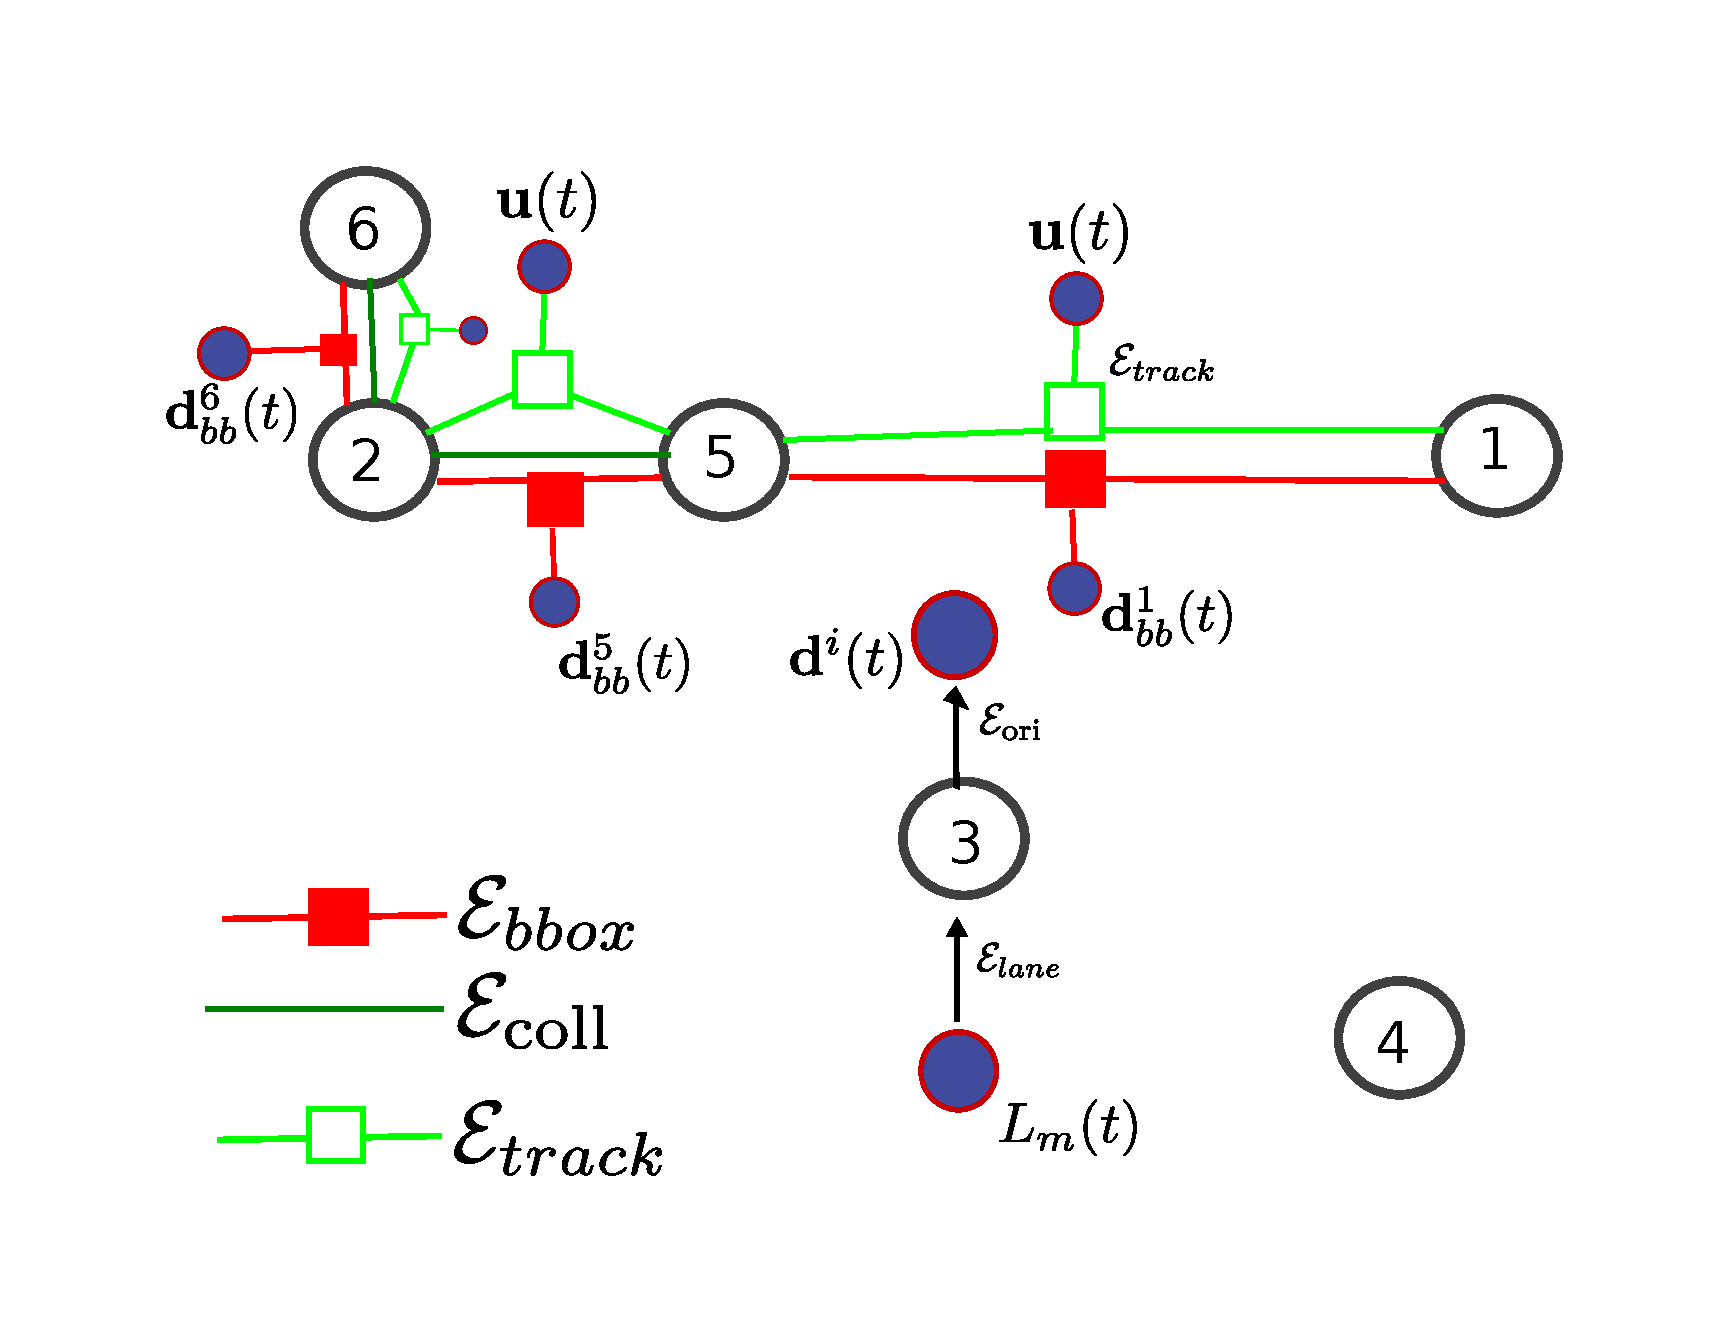
\includegraphics[width=\columnwidth]{graphics/graphicalModelFrom61ConstVars.pdf}
  \caption{Graphical model. The six numbered black circles represent the
    unknown state variables of each car. All other nodes in the graphical model
    are assumed
    observed variables. Consider each energy in the model one by one. (1)
    Bounding box energy: The bounding box energy without occlusion modeling is
    a unary term, but with occlusion it becomes a higher order term that
    affects the state of occluder as well. In this graphical model we assume
    that the scene is being observed from left to right, hence "2" occludes "6"
    and "5" and "5" occludes "1". The bounding box detection is represented by
  $\mathbf{d}_{bb}^i(t)$ and the statistical dependencies are represented by
  red lines. (2) Point tracks ($\Energy{track}$): Since occlusion is also
  included in modeling point tracks energy we have similar interdependencies
  for point tracks energy. The available point tracks are modeled by
  $\mathbf{u}(t)$. (3) Collision ($\Energy{coll}$) : The collision energy
  mathematically is a dense graph between all the TP but here we represent
  collision among only those TP that are near enough to have a significant
collision energy. (4) Orientation from detection ($\Energy{ori}$) (5) Orientation from lane (and map) information ($\Energy{lane}$)}
  \label{fig:graphmodel}
\end{figure}

Assume conditional independence according to graphical model in
\ref{fig:graphmodel}.

\begin{multline}
  P(\{\state{i}{t}\} | \mathbb{E}) =
  \frac{1}{Z}
  \prod_{t=s_i}^{e_i}\prod_{i,j: i \ne j}(P(\state{i}{t}, \state{j}{t}))\\
%
  \prod_{i=1}^{N}
  \prod_{t=s_i}^{e_i}
  P(\bb{i} | \state{i}{t})
  P(\trackp{t} | \state{i}{t})\\
  P(\state{i}{t} | L_m(t))
  P(\state{i}{t} | \state{i}{t-1})
  P(\state{i}{t})
\end{multline}

We can formulate similar objective function in negative log domain:
\footnote{TODO:Resolve inconsistency in summation absorption in energy terms.}
\begin{multline}
  -\log{P(\{\state{i}{t}\} | \mathbb{E})} = 
  Z' + \sum_{i,j:i\ne j} \sum_{t=s_i}^{e_i}  \WEnergyCol \\
  + \sum_{i=1}^N \sum_{t=s_i}^{e_i}
    \WEnergy{box}
  + \WEnergy{track}\\
  + \WEnergy{lane}
  + \WEnergy{dyn}
  + \WEnergy{prior}
\end{multline}

\subsection{Collision energy}

Bhattacharya coefficient $\int_a^b\sqrt{p(x)q(x)}dx$ is a measure of similarity of two
distributions $p(x)$ and $q(x)$. If we represent traffic participants as
gaussians in BEV, then similarity is a measure of collision. Exactly
overlapping distribution results in coefficient as 1. The analytical form of
Bhattacharya coefficient has been taken from
\url{http://like.silk.to/studymemo/PropertiesOfMultivariateGaussianFunction.pdf}

\begin{align}
  \label{eq:collisionEnergyHellingerDistance}
  \EnergyCol &=
  \frac{|\Sigma_i|^\frac{1}{4}|\Sigma_j|^\frac{1}{4}}
  {|P|^\frac{1}{2}}
  e^{-\frac{1}{8}
    \left(\pos{i}{t} - \pos{j}{t}\right)^\top
    P^{-1}
    \left(\pos{i}{t} - \pos{j}{t}\right)
    }
\end{align}
where 
\begin{align}
  P &= \frac{1}{2}\Sigma_i + \frac{1}{2}\Sigma_j\\
\Sigma_i^{-1} &= R^\top_{\ori{i}{t}} \begin{bmatrix} 2/l^i & 0 \\ 0 & 2/w^i \end{bmatrix}
R_{\ori{i}{t}}
\end{align}

\begin{comment}
  \subsection{Bounding box energy}
  \label{sec:totalBBoxEnergy}
  With abuse of notation we represent the four sides of hypothesized bounding
  box by $\projectionOf{\dimsn{i}}$ and detected bounding box by $\bb{i}$.
  Suppose the bounding box $i$ is occluded by bounding box $i$ then the
  bounding box energy becomes a pairwise term.

  \begin{multline}
    \pEnergy{occ}(\relp{i}{t}, \dimsn{i}, \relp{j}{t}, \dimsn{j}) = \\
    \sum_s \rho^{ijs}(t)\projectionOf{\dimsn{i}}_s - \bb{i}_s
               %\sum_{i=1}^N \sum_{t=s_i}^{e_i}
    %\sum_kp_{ik}^{\text{track}}(\projectionOf{\dimsn{i}} - \bb{k})^\top \pmb{\rho}(i,j,t)
  \end{multline}
  where $\rho^{ijs}(t)$ is the visibility fraction of the side $s$ of the
  bounding box. We need to compute visibility fraction we need to compute the
  occlusion mask which is explained in next few sections.

  \subsubsection{Visible faces from bounding boxes}

  \begin{figure}[h]
    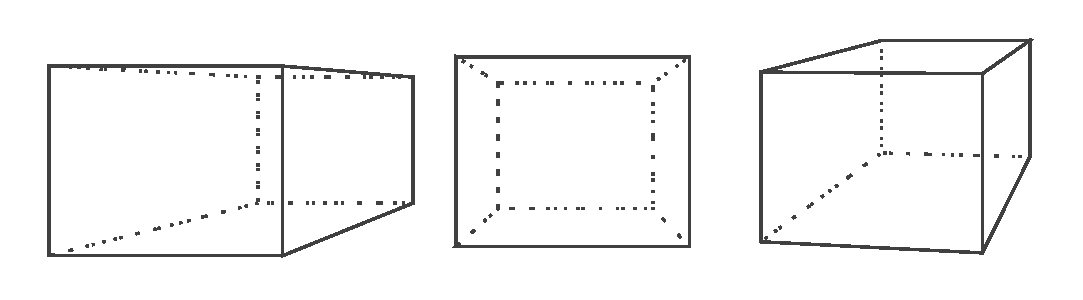
\includegraphics[width=\columnwidth]{graphics/maxFacesVisible.pdf}
    \caption{Only three faces can be visible out of six faces of a bounding
    box.}
  \end{figure}

  \newcommand{\minx}{x_{\text{min}}}
  \newcommand{\miny}{y_{\text{min}}}
  \newcommand{\maxx}{x_{\text{max}}}
  \newcommand{\maxy}{y_{\text{max}}}
  \newcommand{\frontface}{F^i_\text{FF}(t)}
  Each bounding box has 6 faces of which only 3 can be visible.
  Sort the vertices in increasing order of depth. The closest vertex has three
  neighboring faces. All the faces that are visible must be a subset of these
  three. Use first three vertices to
  define the front face (say $\frontface$). Also identify the four 3D points
  that correspond to min/max in x and y direction in the image. If all min-max 4
  points are same as vertices of $\frontface$, then we have only one plane
  visible. If $\{\minx, \maxx\} \not\subset \frontface \land \{\miny, \maxy\}
  \not\subset \frontface$ then we have 3 planes visible. Otherwise we have just
  two planes visible. Let number of planes visible be $n_F$.

  \begin{align}
    n_F &= \begin{cases}
    1 & \text{if }\{\minx, \maxx, \miny, \maxy\} =
    \frontface\\
    2 & \text{else if }\{x_{\text{min}}, x_{\text{max}}\} \subset \frontface \lor
    \{y_{\text{min}}, y_{\text{max}}\} \subset \frontface
    \\
    3 & \text{else if }\{x_{\text{min}}, x_{\text{max}}\} \not\subset \frontface \land
    \{y_{\text{min}}, y_{\text{max}}\} \not\subset \frontface
    \end{cases}
    \label{eq:nfaces}
  \end{align}

  First vertex restrict possible visible faces to three faces. If $n_F = 3$,
  then all three of these faces are visible. If $n_F = 2$, use second closest
  vertex to restrict visible faces to just two. If $n_F = 3$, then front face 
  $\frontface$ is the only visible face.
\end{comment}

\newcommand{\occ}[1]{o({#1})}
\newcommand{\face}{F^i_k(t)}
\begin{comment}
  \subsubsection{Occlusion mask}
  % Initialize empty mask polygon $\occ{0}$ at depth $d=0$.
  % \begin{itemize}
  %   \item Sort all cars in increasing order of depth
  %   \item for each car $i$ in the sorted list
  %     \begin{itemize}
  %       \item Update mask polygon: \\
  %         $\occ{\relpz{i}{t}} = \occ{d} \cup \projectionOf{\dimsn{i}}$
  %       \item $d = \relpz{i}{t}$
  %     \end{itemize}
  % \end{itemize}

  % Sort all planes in increasing order of depth.  This yields a cumulative
  % occlusion mask function
  Occlusion mask is a function that takes the relative depth $d$ from the car
  camera and returns a binary mask that represents occlusions untill that depth.
  Near to the camera occlusion mask is all empty (all zeros) and more occlusions
  get added to the mask with distance.

  \begin{align}
    \occ{d} &= \begin{cases}
    \phi & \text{if } 0 < d \le \relpz{1}{t}\\
    \cup_{i=1}^j \projectionOf{F^i} & \text{if } \relpz{1}{t} < d \le \relpz{j+1}{t}
    \end{cases}
    \label{eq:occlusionmask}
  \end{align}

  where $\relpz{j}{t}$ is the depth of the $j$th traffic participant when sorted
  by increasing depth.

  \subsubsection{Algorithm to get faces based occlusion mask}
  \label{sec:occlusionMaskFromOptVector}

  This is an algorithm to compute occlusion mask Eq.\eqref{eq:occlusionmask}. We
  represent the occlusion mask as a set of polygons.

  Initialize empty mask polygon $\occ{0}$ at depth $d=0$.
  \begin{enumerate}
    \item Collect visible faces using Eq.\eqref{eq:nfaces} for all cars
    %\item for each face get its closest and farthest vertex to the camera.
    \item Create a sorted list of faces
    % \item Create a sorted binary tree of
    %   faces indexed by closed vertices.
    \item Loop over list of sorted visible faces
      \begin{enumerate}
        \item Get the face(s) $\{\face\}$ closer to camera than this face
        \item Add the faces to mask polygon (if not already added): \\
          $\occ{\relpz{i}{t}} = \occ{d} \cup \projectionOf{\face}$
        \item $d = \relpz{i}{t}$
      \end{enumerate}
  \end{enumerate}

  To get the occlusion mask for a face use the farthest vertex of the face to
  query $\occ{.}$.

  \subsubsection{Visibility fraction of a side}
  Let the center of the projected hypothesized bounding box be $\centerProj$ and
  the four corners be $\{\cornerProj{k}\}_{k=1}^{4}$ . Each side and the center
  of the bounding box form a triangle, for example $\triangleProj{1,2} =
  \{\cornerProj{1}, \cornerProj{2}, \centerProj\}$. We take the visibility of
  this triangle as a visibility of the side $s = (1,2)$. Hence the visibility
  fraction of side is given by
  \begin{align}
    \rho^{ijs}(t) = \frac{\|\triangleProj{s} \setminus \occ{\relpz{i}{t}}\|}
                         {\|\triangleProj{s}\|}
     \label{eq:bboxEnergyFromOccMask}
  \end{align}
\end{comment}

\begin{comment}
  \subsection{Occlusion free projection}
  Occlusion free projection can be obtained by applying the precomputed occlusion
  mask to the face projection.
  \begin{align}
    \occFreeProj{\face} &= \projectionOf{\face} \setminus
    \occ{\relpz{i}{t}}
  \end{align}

  \subsection{Perspective-visibility fraction}

  Apart from occlusion, we want to account for the perspective affects. When an 
  objects perspective projection is too small, detection and all related
  evidences deteriorate. One way of this is to find out the projection ratio. In
  fact, we can consolidate projection ratio and occlusion ratio in one term if
  we consider the projection of 3D bounding box planes instead of the entire
  bounding box. 

  \begin{align}
    \rho^i_t &= \sum_{k=1}^{n_F}\frac{\relpz{i}{t}^2\|\occFreeProj{F^i_k(t)}\|}{f^2\|F^i_k(t)\|}
  \end{align}

  where $\occFreeProj{.}$ again means occlusion free projection. $f$ is the
  focal length of the camera so that $\frac{f^2}{\relpz{i}{t}^2}\|F^i_k(t)\|$ is
  the area of projected plane if there were no perspective effects.
\end{comment}


\subsection{Continous Point tracks energy with occlusion}
\label{sec:totalContPtTracksEnergy}
We want continuous modeling of occlusion. We model occlusion as a opacity
term. Based on the dimensions $\dimsn{i}$, we can
compute the covariance matrix $\Sigma_i$ as shown in Sec. 
\ref{sec:sigmacomputation}

So far we have modeled our point tracks energy in a non-smooth way:
\newcommand{\invProjectionOf}[1]{\pi^{-1}_{\relp{i}{t-1}}(#1)}
\begin{multline}
  \Energy{traci}(\{ \relp{i}{t} \}_i, \{ \relp{i}{t-1} \}_i, \{\dimsn{i}\}_i ) = \\
    \sum_{i=1}^{N} 
    %\sum_{t = s_i}^{e_i}
    \sum_{j = 1}^{M}
    \int_1^\infty a_j^i(\lambda)\|\trackpj{t} - \projectionOf{\invProjectionOf{\trackpj{t-1}}}\|^2 d\lambda
\end{multline}

The tricky part here is inverse projection $\invProjectionOf{.}$ . When we
project an image point back to 3D we get a ray $\lambda K^{-1}\trackpj{t-1}$
which is ambiguous up to a scale factor $\lambda$. Using our hypothesized 3D
layout of the scene we can estimate this scale factor, we
can compute a distribution over the $\lambda$. 
\subsubsection{Occupancy function}
Assuming occupancy to be a
probability distribution over 3D space. For each traffic participant the
occupancy is modeled as a logistic function 
\newcommand{\occf}{f^i_{occ}(\mathbf{x})}
\begin{align}
   \occf = L(\mathbf{x}; \pos{i}{t}, \Sigma_i)
\end{align}
where $L(.)$ is the logistic function defined by
\begin{align}
  L(\mathbf{x}; \pos{i}{t-1}, \Sigma_i) = \frac{1}{
    1 + e^{-k(1 - d(\mathbf{x},\pos{i}{t-1}))}
    }
\end{align}
where $d(\mathbf{x},\pos{i}{t-1}) =
(\mathbf{x}-\pos{i}{t-1})^\top\Sigma_i(\mathbf{x}-\pos{i}{t-1})$ and $k =
10\ln{49}$. $k$ is chosen such that $L(.) = 0.98$ when $d(.) =
0.9$

We model the probability of a point being projected to a camera is dependent
up two factors, (1) reflection and (2) transmission through intermediate
space. 
\subsubsection{Reflection probability}
For lambertian reflection we replace the surface normal with the
gradient of occupancy.
\begin{align}
  P_{\text{reflection}} = \sum_i (\max \{0, \nabla \occf^\top
  \hat{\mathbf{r}_j}\})^2
\end{align}
where $\hat{\mathbf{r}_j} =
\frac{K^{-1}\trackpj{t-1}}{\|K^{-1}\trackpj{t-1}\|}$ is unit vector in the
direction of ray. The gradient in the direction opposite to ray yields -ve
probability which needs to be clipped off. Squaring the function keep it
smooth near zero.

\subsubsection{Transmission probability}
A model for transmission of light through a material of thickness $x$,
density $\rho$ and opacity $k_o$ is given by Beer-Lambert law 
\begin{align}
  I(x) = I_0e^{-k_o\rho x}
\end{align}

Since both opacity and density are represented by our occupancy function
$\occf$, and also the domain of our $\occf$ is $[0, 1]$ instead of $[0,
\infty]$ as in case of $k_o$; we replace $e^{-k_o\rho}$ by our transparency
function $1 - \occf$. So the transmission probability over a small distance
$d\lambda$ is given by
\begin{align}
  P_{\text{transmission}}(\lambda + d\lambda) =
  P_{\text{transmission}}(\lambda) (1-\occf)^{d\lambda}
\end{align}
\newcommand{\ray}{\hat{\mathbf{r}}_j}
\newcommand{\occfray}{f_{occ}(\lambda\ray)}

For our given ray $\mathbf{x}_j = \lambda \ray$, the probability that the point
$\trackpj{t-1}$ is reflected from a distance $\lambda$ is given by

\newcommand{\lambdadist}{f_{\lambda}(\trackpj{t-1}, \lambda)}
\begin{align}
  \lambdadist &= P_{\text{reflection}}
  \prod_{0}^{\lambda} (1 - f_{occ}(\lambda \ray))^{d\lambda} %\\
  %= \max \{ 0, (\nabla f_{occ}&(\lambda \ray)^\top \ray) \}
  %\prod_{0}^{\lambda} (1 - f_{occ}(\lambda \ray))^{d\lambda}
\end{align}
where $\prod_{0}^{\lambda}$ represents the \emph{product integral} from $0$ to
$\lambda$. A product integral is a simple integral in log domain
\begin{align}
  \prod_{0}^{\lambda} (1 - f_{occ}(\lambda \ray))^{d\lambda} =
  e^{\int_{1}^{\lambda} \ln{(1 - f_{occ}(\lambda \ray))}{d\lambda}}
\end{align}

% Once we have our distribution over $\lambda$, $\lambdadist$ we can compute the
% reprojection of $\trackpj{t-1}$ over image in time $t$ as a function of
% $\lambda$. Let

\subsubsection{Reprojection error}

\begin{align}
  f^{i}_{reproj}&(\trackpj{t-1}, \lambda) =
  \projectionOf{\invProjectionOf{\trackpj{t-1}}}\\
  %&= K(R^i_t ((R^i_{t-1})^\top\lambda \ray - (R^i_{t-1})^\top T_{t-1}) + T_{t})\\
  &= \frac
  {p_{1:2}\lambda + q_{1:2}}
  {p_{3}\lambda + q_{3}}
\end{align}
where $p_{1:3} = KR^i_t(R^i_{t-1})^\top\ray$ and
$q_{1:3} = KR^i_t(R^i_{t-1})^\top T_{t-1} + KT_t$

Now that we have an association from TP $i$ to point track $j$ through
$\lambda$, we can come up with an association probability
\newcommand{\occfxi}{L(\mathbf{x}; \pos{i}{t-1}, \Sigma_i)}
\newcommand{\occfi}{L(\lambda \ray; \pos{i}{t-1}, \Sigma_i)}
\newcommand{\assocP}{a^{i}_{j,t-1}(\lambda)}
\newcommand{\assocPk}{a^{i}_{j,t-1}(\lambda_k)}
\begin{align}
   \assocP &= \frac{(\max \{ 0, \nabla \occf^\top
\ray \})^2 }{P_{\text{reflection}}}\lambdadist\\
&=(\max \{ 0, \nabla \occf^\top \ray \})^2
  \prod_{0}^{\lambda} (1 - f_{occ}(\lambda \ray))^{d\lambda}
\end{align}

Note that this fraction although called association probability does not
capture the entire information that we have available for compute association
of points to tracks. This above fraction is the association probability given 
the hypothesized parameters of traffic participant model. Given that a point is
observed on the image the sum of probability marginalized over other parameters
must be one i.e.
\begin{align}
    \sum_{i = 1}^N
    \int_1^{\infty}
    \assocP d\lambda = 1
\end{align}

To compute the association probability between traffic participant $i$ and
point track $j$ we must use re-projection error as well. When the association
$i$ and $j$ is right and the point of reflection is at depth $\lambda$ the
re-projection error must be zero, otherwise the error becomes a measure of
distance from the true solution:

\newcommand{\Ereproj}{E^{(ij)}_{\text{reproj}}}
\begin{align}
  \Ereproj(\lambda) = \|\trackpj{t} - f^i_{reproj}(\trackpj{t-1}, \lambda)\|^2
\end{align}

The error terms can be converted to probability domain by considering the error
term as negative log of probablity

\begin{align}
  P^{(ij)}_{\text{assoc by reproj}}(\lambda) = \frac{1}{\sqrt{2\pi}}\exp(-\Ereproj(\lambda))
\end{align}

Using both the evidence terms we can write probability of association as
\begin{align}
  P^{(ij)}_{\text{assoc}} \propto \int_0^{\infty} \assocP \frac{1}{\sqrt{2\pi}}\exp(-\Ereproj(\lambda))d\lambda
  \label{eq:prob-assoc}
\end{align}

However, for estimating the overall energy we just need to compute the expected
value of the re-projection error for given parameters, i.e.

\begin{multline}
  \Energy{track}(\{ \relp{i}{t} \}_i, \{ \relp{i}{t-1} \}_i,\{ \dimsn{i} \}_i) = \\
    \sum_{i = 1}^N
    \sum_{j = 1}^{M}
    \int_1^{\infty}
    a^i_{j,t-1}(\lambda) 
    \|\trackpj{t} - f^i_{reproj}(\trackpj{t-1}, \lambda)\|^2
    d\lambda
\end{multline}

If the aim is to find the best possible association, it is easier as we need to
to compute the association that minimizes the expected re-projection error for
point $j$. It remains to be seen that how the minima of following expression relates to minima of \eqref{eq:prob-assoc}

\begin{align}
  i^* = \argmin_{i=1}^N \int_0^\infty \assocP \Ereproj(\lambda) d\lambda
\end{align}

Since the computation of $\assocP$ entirely depends on hypothesized parameters,
it severely limits the applicability of this method outside this kind of
parameterized model.

\subsubsection{Approximations}
\newcommand{\Ptrans}{P_{\text{transmission}}}
\newcommand{\Prefl}{P^i_{\text{reflection}}}
\newcommand{\dishort}{d_i(\mathbf{x})}

Reflection probability of $i$th traffic participant is easy to compute
analytically 
\begin{multline}
  \Prefl =
  (\max \{ 0, \nabla \occf^\top \ray \})^2 \\
  = (\max \{ 0, \nabla \occfxi^\top\ray \})^2
  \label{eq:analytic-prefl}
\end{multline}
where 
\begin{multline}
  \nabla \occfxi^\top\ray \\=
  \nabla k\dishort \sech^2\left(\frac{k}{2}\dishort\right)
\end{multline}
where $\dishort = 1-d(\mathbf{x}, \pos{i}{t-1})$ is a signed distance measure
from the contour of the ellipsoid where $d(\mathbf{x}, \pos{i}{t-1})$ is 1.

However, the transmission probability needs to be approximated.  
%
% \subsubsection{Computing $\Prefl$ and $\Ptrans$}
% Focusing on  $\nabla \occfxi$ 
% 
% \begin{multline}
%   \nabla \occfxi =\\
%   \frac{-k\nabla d(\mathbf{x}, \pos{i}{t-1})e^{-k(1-d(\mathbf{x}, \pos{i}{t-1}))}}{
%     (1 + e^{-k(1-d(\mathbf{x}, \pos{i}{t-1}))})^2
%   } \\ 
%   = -k\nabla d(\mathbf{x}, \pos{i}{t-1})\sech^2\left(\frac{k}{2}(1-d(\mathbf{x},
%   \pos{i}{t-1}))\right)
%   \\
%   = \nabla k\dishort \sech^2\left(\frac{k}{2}\dishort\right)
% \end{multline}
% where $\dishort = 1-d(\mathbf{x}, \pos{i}{t-1})$ is a signed distance measure
% from the contour of the ellipsoid where $d(\mathbf{x}, \pos{i}{t-1})$ is 1.
% Focusing on $\nabla d(.)$
% 
% \begin{align}
%   \nabla d(\mathbf{x}, \pos{i}{t-1}) = 2\Sigma_i(\mathbf{x} - \pos{i}{t-1})
% \end{align}
% Back to \eqref{eq:analytic-prefl}
% 
% \begin{multline}
%   (\max \{ 0, \nabla \occf^\top \ray \})^2 = \\
%   \sech^4\left(\frac{k}{2}\dishort\right) 
%   (\max \{ 0 , \nabla k\dishort^\top\ray\})^2
% \end{multline}
% 
% The probability is simply $\sech^2(.)$ scaled by gradient of ellipsoid
% $\nabla k\dishort$ projected in the ray direction $\ray$.
% 
% \begin{align}
%   \Ptrans = 
%   e^{\int_{1}^{\lambda} \ln{(1 - f_{occ}(\lambda \ray))}{d\lambda}}
% \end{align}
% \begin{multline}
% \int_{1}^{\lambda} \ln{(1 - f_{occ}(\lambda \ray))}{d\lambda}
% =  \\
% \int_{1}^{\lambda} \ln{\left(1 - \sum_i \occfi\right)}{d\lambda}
% \end{multline}
% 
% The above integral is very difficult to approximate or compute analytically.
So based on intuition, we approximate the $\Ptrans$ by following function
\begin{align}
\label{eq:evalCumulativePtrans}
  \Ptrans &= \prod_i L_u(\mathbf{u}, \mu^i_u,\Sigma^i_u)L_{\lambda}(\lambda; \mu^i_d)\\
  L_u(\mathbf{u}, \mu^i_u,\Sigma^i_u) &= \frac{1}{
    1 + e^{-k_u(1 - (\mathbf{u} - \mu^i_u)^\top\Sigma^i_u(\mathbf{u} -
    \mu^i_u))}
  }
  \\
  L_{\lambda}(\mathbf{u}, \lambda; \mu^i_d) &= \frac{1}{
  1 + e^{-k_d(\lambda - \mu^i_d(\mathbf{u}))}
}
\end{align}
where 
\begin{align}
  \mu_u^i &= \projectionOf{\pos{i}{t-1}} \label{eq:muiudef}\\
  \Sigma_u^i &= \projectionOf{\Sigma_i} \label{eq:sigmauidef}\\
  \mu^i_d(\mathbf{u}) &= \relp{i}{t}\\
  k_u &= 10\log(49)\\
  k_d &= \frac{\log(49)}{\sqrt{h^2 + l^2 + w^2}}
  \label{eq:ptransmissionInit}
\end{align}
is the distance of the centre of the traffic participant from the camera.

% $\mu^i_d(\mathbf{u}) = \min_{\lambda} d^2_i(\lambda K^{-1}\mathbf{u})$.
% $\mu^i_d(\mathbf{u})$ is the closest point to the unit contour of ellipsoid.
% If there are multiple such points, the point closest to the camera is taken as
% $\mu^i_d(\mathbf{u})$

The association probability becomes

\newcommand{\Lu}{L_u(\mathbf{u}, \mu^i_u,\Sigma^i_u)}
\newcommand{\Llambda}{L_{\lambda}(\mathbf{u}, \lambda; \mu^i_d)}
\begin{multline}
  \assocP = 
    \sech^4\left(\frac{k}{2}\dishort\right)
    (\max \{ 0, \nabla k\dishort^\top\ray \})^2\\
  \prod_i \Lu
    \Llambda \\
    \label{eq:assocCoeffEval}
\end{multline}

So the energy becomes

\begin{multline}
  \label{eq:integrand}
  \Energy{track}(.) = 
    \sum_{i = 1}^N
    \sum_{j = 1}^{M}
    \int_1^{\infty}
    \assocP
    \Ereproj(\lambda)
    d\lambda
\end{multline}
where $x = \lambda \ray$ and $\Ereproj(\lambda) = \|\trackpj{t} -
f^i_{reproj}(\trackpj{t-1}, \lambda)\|^2$ is reprojection error which is a
quadratic in $\lambda$

The integral in the above expression is computed numerically.

\subsection{Numerical integration}
Numerical integration is possible by computed by sampling. Samples need to be
generated from the association probability $\assocP$ for a given $j$. We take
proposal distribution to be a GMM with modes around probable reflection points.
The weights of all Gaussians in the mixture are proportional to the distance of
the point $j$ from projection of ellipsoid centre i.e. 
\begin{align}
  A_{ij} = \frac{1}{Z_j}\exp(-(\trackpj{t} - \mu^i_u)^\top\Sigma_u^i(\trackpj{t} - \mu^i_u))
\end{align}
where $Z_j = \sum_{i=1}^N A_{ij}$ and $\mu^i_u$ and $\Sigma_u^i$ are described in \eqref{eq:muiudef} and \eqref{eq:sigmauidef} respectively.
The range of Gaussian $G_i$
must be in the interval $[\|\relp{i}{t}\|, \|\relp{i}{t}\| -
\sqrt{3}\max(\dimsn{i})]$. Hence we take the mean as $\|\relp{i}{t}\| -
\frac{\sqrt{3}}{2}\max(\dimsn{i})$ and variance as
$\frac{1}{3}\max(\dimsn{i})^2$. The distribution from which we sample is 
\newcommand{\Gauss}{\mathcal{N}}
\newcommand{\PropDist}{\mathcal{W}_j}
\begin{align}
  \PropDist(\lambda) = \sum_i A_{ij} \Gauss(\lambda; \|\relp{i}{t}\| -
  \frac{\sqrt{3}}{2}\max(\dimsn{i}), \frac{1}{\sqrt{3}}\max(\dimsn{i}))
\end{align}
And the numerical integral with $K$ samples is computed by
\begin{align}
    \int_1^{\infty}
    \assocP
    \Ereproj(\lambda)
    d\lambda
    =
    \frac{1}{K}\sum_k \Ereproj \frac{\assocPk}{\PropDist(\lambda_k)}
\end{align}
where $\lambda_k$ is the $k$th sample drawn from $\PropDist(\lambda)$.

\begin{comment}
  %%%%%%%%%%%%%%%% Analytical attempt to integration %%%%%%%%%%%%%%%%%%%%%
  \begin{align}

    E^i_{\text{reproj}}(\lambda) &= \left\|\trackpj{t} - \frac{p_{1:2}\lambda +
  q_{1:2}}{p_3\lambda + q_3}\right\|^2\\
  &= \frac{(p_1\lambda + q_1 - u_{j1}(t))^2 + (p_2\lambda + q_2 - u_{j2}(t))^2}
  {(p_3\lambda + q_3)^2}\\
  &= \frac{a\lambda^2 + b\lambda + c}{(p_3\lambda + q_3)^2}
  \end{align}
  where $a = p_1^2 + p_2^2$, $b = 2p_1(q_1 - u_{j1}(t)) + 2p_2(q_2 - u_{j2}(t))$
  and $c = (q_1 - u_{j1}(t))^2 + (q_2 - u_{j2}(t))^2$

  So, in terms of $\lambda$ we have the integrand as
  \begin{multline}
    \int_1^\infty
    \prod_i (1 +
    \tanh(\poly^{(1)}_{ij1}(\lambda)))\sech^4(\poly^{(2)}_{ij2}(\lambda))\\
    (\max\{ 0, \poly^{(2)}_{ij3}(\lambda) \})^2
    \frac{\poly^{(2)}_{ij4}(\lambda)}{(\poly^{(1)}_{ij5}(\lambda))^2}d\lambda
  \end{multline}
  where $\poly^{(n)}_{ijk}$ denotes a polynomial $k$ of order $n$ dependent upon $i$th
  traffic participant and $j$th point. This integrand is still too difficult to
  be solved or approximated analytically.

  We approximate the expression,

  \begin{multline}
    \prod_i \Llambda
  \sech^4\left(\frac{k}{2}\dishort\right)(\max\{ 0, \nabla k\dishort^\top\ray \})^2
  \end{multline}

  with a
  gaussian with mean at $\mu^{ij}_{\lambda} : d_i(\mu^{ij}_{\lambda}\ray) = 0$
  standard deviation as $\sigma^{ij}_{\lambda} =
  \frac{\pi}{2\sqrt{3}kd(\mu^{ij}_{\lambda}\ray, \pos{i}{t-1})}$  and magnitude as the
  expression computed at mean. An integrand of the form
  \begin{align}
    \frac{\poly^{(2)}_{ij4}(\lambda)}{(\poly^{(1)}_{ij5})^2}
      e^{\frac{- (\lambda -
  \mu^{ij}_{\lambda})^2}{\sigma^{ij}_{\lambda}}}
  \end{align}
   is integrable analytically by parts.

   \newcommand{\muijl}{\mu^{ij}_{\lambda}}
   \newcommand{\sigmaijl}{\sigma^{ij}_{\lambda}}
   \begin{align}
   \int_1^\infty \frac{a\lambda^2 + b\lambda + c}{(p_3\lambda + q_3)^2}e^{\frac{- (\lambda -
  \mu^{ij}_{\lambda})^2}{\sigma^{ij}_{\lambda}}}d\lambda
   \end{align}
   Substituting $y = \frac{\lambda - \mu^{ij}_{\lambda}}{\sigma^{ij}_{\lambda}}$

   \begin{align}
     \int_1^\infty \frac{a_y y^2 + b_yy + c_y}
     {(p_{3y}y + q_{3y})^2}e^{-y^2}dy
   \end{align}
   where $a_y = a(\sigmaijl)^3$, $b_y = (2a\muijl + b)(\sigmaijl)^2$ and $c_y =
   (2a(\muijl)^2 + b\muijl + c)\sigmaijl$ and $p_{3y} = \sigmaijl p_3$ and
   $q_{3y} = p_3\muijl + q_3$


  % \subsubsection{Sandwich of ellipsoids model}
  % 
  % \begin{enumerate}
  %   \item Model $\occf$ as
  %     sigmoid over ellipse instead of a gaussian.
  %     \begin{align}
  %       \occf = \frac{1}{
  %       1 + e^{-(\mathbf{x} - \pos{i}{t})^\top
  %         \Sigma_i (\mathbf{x} - \pos{i}{t}))}}
  %     \end{align}
  %   \item To get the intuition of this occupancy function imagine the traffic
  %     participant as layered ellipsoid. The innermost ellipsoid has very high
  %     probability (approx 1) of being occupied. The outermost ellipsoid has very
  %     low probability (approx 0) of being occupied. We will just consider the
  %     occupancy interplay within these two ellipsoids.
  %   \item Project outer ellipsoids of all TP's on the image.
  %   \item Consider the ellipses that bound the track point $\trackpj{t-1}$.
  %   \item For each ellipse do
  %     \begin{itemize}
  %       \item Case 1: The ray intersects inner ellipse
  %         Now the ray intersects both inner and outer ellipse
  %         Compute the intersection points on both the ellipses
  %         Compute the gradient function $\nabla\occf^\top \ray$ at
  %         the mid point of the two intersections. Use this as the magnitude of
  %         gaussian mixture component centered at the mid point of intersections
  %         and spread such that 97 percentile of probability mass of guassian is
  %         within the intersection points. With the same parameters model the
  %         transimission probability with product of logistic function $L(.)$.
  %       \item Case 2: The ray do not intersects inner ellipse.
  %         The ray just passes through the outer ellipse. Find the point on the
  %         ray closest to the center of the ellipse. Compute gradient function
  %         at the closest point, which will be again used as the magnitude of
  %         gaussian mixture component centered at the closest point and spread
  %         such that 97 percentile of probabiltiy mass of gaussian is within the
  %         two intersection points of the ellipse. With the same parameters model
  %         the transimission probability with product of sigmoids.
  %     \end{itemize}
  %   \item Now this approximated $\lambdadist = \sum N(.) \prod (1 - L(.))$ can
  %     be used in integrating the error over $\lambda$.
  % \end{enumerate}
  \newpage

  \clearpage
  %%%%%%%%%%%%%%%% Analytical attempt to integration %%%%%%%%%%%%%%%%%%%%%
\end{comment}

\subsubsection{Sigma of ellipsoid}
\label{sec:sigmacomputation}

\newcommand{\Sigmait}{\Sigma^i_t}
\newcommand{\muit}{\mu^i_t}
\begin{align}
  \muit &= \begin{bmatrix}
  0& 0& \frac{h}{2}
  \end{bmatrix}^\top\\
  \Sigmait &= \begin{bmatrix}
    \frac{4}{l^2} & 0 & 0 \\
    0 & \frac{4}{w^2} & 0 \\
    0 & 0 & \frac{4}{h^2}
  \end{bmatrix}
\end{align}

In tracklet coordinates the equation of ellipsoid is 
\newcommand{\xt}{\mathbf{x}_t}
\newcommand{\xc}{\mathbf{x}_c}
\begin{align}
  (\xt - \muit)^\top \Sigmait (\xt - \muit) = 1
\end{align}


Moving to camera coordinates
\newcommand{\Rctot}{R}
\newcommand{\tctot}{t}
\begin{align}
  (\Rctot \xc + \tctot - \muit)^\top \Sigmait (\Rctot \xc + \tctot - \muit) = 1
\end{align}

\newcommand{\tcmut}{t'}
Let $\tcmut = \tctot - \muit$
\begin{align}
  (\Rctot \xc + \tcmut)^\top \Sigmait (\Rctot \xc + \tcmut) = 1
\end{align}
\begin{align}
  \xc^\top \Rctot^\top \Sigmait \Rctot \xc + 2 (\Rctot^\top \tcmut)^\top  \Rctot^\top\Sigmait \Rctot \xc
  + \tcmut^\top \Sigmait \tcmut = 1
\end{align}
\newcommand{\Sigmaic}{\Sigma'^i_c}
\newcommand{\muic}{{\mu^i_c}}
Let $\Sigmaic = \Rctot^\top \Sigmait \Rctot$ and $\muic = - \Rctot^\top
\tcmut$
\begin{align}
  (\xc - \muic)^\top\Sigmaic(\xc - \muic) - \muic^\top\Sigmaic\muic +
  \tcmut^\top \Sigmait \tcmut = 1
\end{align}
\newcommand{\Sigmaicf}{\Sigma^i_c}
Let $\Sigmaicf = \frac{\Sigmaic}{1 - \tcmut^\top \Sigmait \tcmut +
\muic^\top\Sigmaic\muic}$
\begin{align}
(\xc - \muic)^\top\Sigmaicf(\xc - \muic) = 1
\end{align}

Hence, we have following expression for mean and sigma of ellipsoid:
\begin{align}
  \label{eq:ellipsoidMeanSigma}
  \muic &= - \Rctot^\top \tcmut \\
  \Sigmaicf &= \frac{\Sigmaic}
{1 - \tcmut^\top \Sigmait \tcmut + \muic^\top\Sigmaic\muic}
\end{align}


% \subsection{Object detection score}
% \begin{align}
% \Energy{det}(\relp{i}{t}, \dimsn{i}) = 
%              \frac{1}{S_t^2(\projectionOf{\dimsn{i}})}
% \end{align}

% \subsection{Object 2D bounding box with occlusion}
% Reproduced from \cite{song2014eccv} section 4.3
% 
% \begin{multline}
%   \Energy{box}(\relp{i}{t}, \dimsn{i}) =
%              %\sum_{i=1}^N \sum_{t=s_i}^{e_i}
%              \rho^i_t \|\projectionOf{\dimsn{i}} -
%              \bb{i}\|^2
% \end{multline}
% 
% where $S_t(.)$ is the function to approximate the detection scores using
% mixture of Gaussian model and $\rho^i_t$ is the visibility fraction. 
% 
% % It can be
% % computed by using polygon intersection algorithms.
% % \begin{align}
% %   v^i_t &= \frac{\|\occFreeProj{\dimsn{i}}\|}
% %                 {\|\projectionOf{\dimsn{i}}\|}
% % \end{align}
% % where $\|.\|$ represents the norm or the area of the polygon.
% 
% Another approach is to just consider the corner points in the occlusion free
% area.  Say $\projectionOf{\dimsn{i}} = [b^i_1, \dots, b^i_4]$.
% \begin{multline}
%   \Energy{box}(\relp{i}{t}, \dimsn{i}) =
%              %\sum_{i=1}^N \sum_{t=s_i}^{e_i}
%              %S_t^2(\projectionOf{\dimsn{i}})
%              \sum_{{b^i_j} \in \occFreeProj{\dimsn{i}}}
%              \|b^i_j - d^i_j\|^2
% \end{multline}
% 
% In the opinion of this author, the second approach is better because the
% visibility is an area based measure while the error metric is point to point
% distance based measure. If we use bounding overlap instead of corner to corner
% distance, the use of visibility fraction makes much more sense. However, one
% can argue that even detection score is an area based measure. 
% 
% Hence a third approach can be 
% \begin{multline}
%   \Energy{box}(\relp{i}{t}, \dimsn{i}) =
%              %\sum_{i=1}^N \sum_{t=s_i}^{e_i}
%   \rho^i_t \|\projectionOf{\dimsn{i}} \ominus \bb{i}\|
% \end{multline}
% where $A \ominus B$ represents the symmetric difference between set $A$ and set
% $B$ and is given by $A \ominus B = (A \cup B) \setminus (A \cap B)$.
% One may argue that we can take the intersection of occlusion free projection 
% and get rid of the visibility fraction, but that would be a little off the 
% detection bounding box is usually more close to the projection of full car
% instead of the just the visible portion.
% 
% 
% \subsection{Orientation cues}
% There are two orientation cues (1) orientation from detection (2) orientation
% from appearance map \cite{yao2012describing}.
% 
% \begin{align}
%   \Energy{ori} &= 
%   %S_t^2(\projectionOf{\dimsn{i}})
%   \rho^i_t(1 - \cos({\omega}^i_{\text{det}} - \ori{i}{t})
% \end{align}
% 
% Appearance map is a shape prior that requires \emph{Scene labeling} input.

\section{Continuous object detection score energy with occlusion} 

To start with we have hypothesized 3D bounding boxes $\{ \dimsn{i} \}_i$
over all traffic participants and we have object detection scores modeled as
mixture of Gaussians over four dimensional space of bounding box boundaries.
Let the detection score function over the detection $\bb{i}$ be 
%
\begin{align}
  S(\bb{i}) = \sum_j A_j \exp((\bb{i}-\mu^{(d)}_j)^\top \Sigma^{(d)-1}_j
  (\bb{i}-\mu^{(d)}_j))
\end{align}
%

\subsection{Soft occlusion regions}
The soft occlusion regions is exactly the $\Ptrans$
%
\begin{align}
  O_{j}(x; \mu_{Oj}, \Sigma_{Oj}) = 1 - \Ptrans
\end{align}
%

\subsection{Merging occlusion regions with detection score}
What does detection score function represents? It is a measure of
correlation of trained object features and the features in the candidate
bounding box. If the detection scores are indeed Gaussians around the mean
bounding box $\mu_j$, the $\Sigma_j^{-1}$ represents the variance (and
covariance) around the mean bounding box. But when the candidate objects seem
to be occluded we have additional information available. In such a case, we
can say that the occluded object might have unexpected effect on the detection
scores. However, the uncertainty in the detection score in loop sided. The
mean detection bounding box must have picked up correct boundaries on the
un-occluded sides but we cannot say the same about occluded boundaries. The
effect on detection score depends a lot on the features of the occluder. Given
this understanding we want to decrease our confidence on the mean detection
boundaries around the occluded boundaries. One of the simplest ways will be to
scale the appropriate diagonal element of $\Sigma_j$ by an appropriate scaling
factor. But how does occlusion affects the non diagonal terms. Consider that we
have a set of measurements whose mean and variance are known $\mu = E(x)$ and $\Sigma = E ((x - \mu_x)(x - \mu_x)^\top)$. We want to know the
affect of uncertainty on mean and variance of existing observations. On adding
noise $[\Delta x, \Delta y]^\top$ with zero mean and covariance $\Delta
\Sigma = E(\Delta x \Delta x^\top)$ the covariance of new data is given by
\begin{multline}
  E((x + \Delta x)(x+\Delta x)^\top) = E(xx^\top) + E(x \Delta x^\top) \\
  + E(\Delta x x^\top) + E(\Delta x \Delta x^\top)
\end{multline}
where the terms $E(x \Delta x^\top)$ denote the correlation between the data
vector and the uncertainty in the data. Although we understand that in our case
the data is the appearance based detection score and uncertainty because of
occlusion is closely related to the appearance and hence detection score, we
assume independence between $x$ and $\Delta x$. Hence our resultant covariance
matrix $ E((x + \Delta x)(x+\Delta x)^\top) = \Sigma + \Delta \Sigma$

We observe that the soft occlusion regions are 2D while the detection scores
are 4D. But that should not be a problem because the detection scores are
modeled as $[x_{\text{min}}, y_{\text{min}}, x_{\text{max}},
y_{\text{max}}]^\top$, we can stack the vectors in the soft occlusion region
domain as the regions are independent of min or max variation. The parameters
of 4D occlusion distribution are given by

\begin{align}
  \mu'_{Oij} = [\mu_{Oij}^\top \mu_{Oij}^\top]^\top
  \Sigma'_{Oij} = \begin{bmatrix}
    \Sigma_{Oij} & \Sigma_{Oij} \\
\Sigma_{Oij} & \Sigma_{Oij}
  \end{bmatrix}
\end{align}

With our
discussion so far, the function $O_{ij}(.)$ gives an additional measure of
uncertainty associated with each point in the space. To finally re-model our
detection scores scaled by continuous occlusion we sample $O_{ij}(.)$ at the
mean detection boundaries from GMM $S(.)$ and we scale the detection boundary
variance by $\mathcal{P}_{j} = \rho_{j}\rho_{j}^\top$ where $\rho_{j} =
O_{j}(\mu^{(d)}_i; \mu'_{Oj}, \Sigma'_{Oj})$. The new variance
in detection score is given by 
%
\begin{align}
  \Sigma'^{(d)}_j = \mathcal{P}_{j}
  + \Sigma^{(d)}_j
\end{align}
%
The detection scores GMM with occlusion is given by replacing the covariance
matrix
\begin{align}
  S'(\bb{i}) = \sum_j A_j \exp((\bb{i}-\mu^{(d)}_j)^\top \Sigma'^{(d)-1}_j
  (\bb{i}-\mu^{(d)}_j))
\end{align}

\newcommand{\Beizer}{B\'eizer }
\subsection{Lane energy}
\label{sec:laneEnergy}
 The lanes be are modeled as splines. The lanes geometry information can be
 obtained from camera input as well as from the available maps localized by
 GPS. We need to combine information in a different framework to lead to a
more accurate solution by using both the sources. In a probablistic framework
it is always useful to compute uncertainty along the estimated values.
Here we assume that the confidence in lane detection is inversely proportional
to the squre of distance of of the specific point on the lane to the camera
\newcommand{\LaneUncertainty}[1]{\Sigma_{L_m}(#1)}
$\Sigma_{L_m}({x}_{L_m}) = \frac{1}{\|\mathbf{x}_{L_m} - \egop\|^2}$.

A lane is modeled by four control points of a \Beizer curve $L_j = \{l_0, l_1,
l_2, l_3\}$. The parametric curve is given by $L_j(k) = \sum_{i=0}^3 {}^3C_i
(1-t)^{3-i}t^i l_i$. \Beizer are double differentiable so one can find
tangents ($L'_j(k)$) and normals $R_{\frac{\pi}{2}}L'_j(k)$ where 
$R_{\frac{\pi}{2}} = \begin{bmatrix} 0 & -1 \\ 1 & 0 \end{bmatrix}$ is
$90^\circ$ rotation matrix.

\newcommand{\projOnLane}[1]{\pi_{L_m(k)}(#1)}
Now, there are some algorithms \cite{ma2003point, chen2007improved} to
approximate the closest point on a \Beizer curve $k_x = \projOnLane{x}$.
Consequently one can get solutions for shortest distance $s =
\text{DIST}(L_j(k), x)$ and orientation at a closest point on the lane
$\mathbf{t} = \text{TAN}(L_j(k), x)$.

% \subsubsection{Position in lane}
%
% \begin{align}
%   \Energy{plane} &=
%   \min_{j = 0}^{n_l} \text{DIST}(L_j(k), \pos{i}{t})
% \end{align}
%
 % 
 % We normalize it with the confidence in lane positions.
 % 
 % \begin{align}
 %   \Energy{plane} &=
 %   \min_{m = 0}^{n_l} \text{DIST}(L_m(k), \pos{i}{t})
 %   \LaneUncertainty{\pos{i}{t}}
 % \end{align}



\subsubsection{Orientation within lane}
\begin{itemize}
  \item We can find the tangent to a lane
  \item The energy is given by the dot product between car orientation
    and tangent to the lane at that point.
\end{itemize}

% \begin{align}
%   \Energy{olane} &= 1 - \text{TAN}(L_l(k),  \pos{i}{t})
%   \cdot
%   \ori{i}{t}
% \end{align}
% 
% 
% 
% This model needs to be scaled by uncertainty. For example, if we want to say
% that the farther the lane is from the camera we are less sure about lane
% orientation and hence this evidence term we scale it by say square of distance
% of the car position from camera.

% \begin{align}
%   \Energy{olane} &= 
%   (1 - \ori{i}{t} \cdot \text{TAN}(L_{m^*}(k),  \pos{i}{t}) )
%   
% \end{align}
% where $m^* = \arg \min_m \text{DIST}(L_m(k), \pos{i}{t})$

\begin{align}
  \label{eq:laneOrientationEnergy}
  \Energy{lane} &= 
  \sum_{m \in M_{\text{close}}}
  (1 - \ori{i}{t} \cdot \text{TAN}(L_{m}(k), \pos{i}{t}) )
\LaneUncertainty{\pos{i}{t}}
\end{align}
where $M_{\text{close}} = \{m : \text{DIST}(L_{m}(k), \pos{i}{t}) < 50\} $ is
the set of nearby lanes and 
\begin{align}
\LaneUncertainty{\pos{i}{t}} = 
  \frac{1}{1 + exp(-q(w_{\text{road}} - \text{DIST}(L_{m}(k), \pos{i}{t})))}
\end{align}
for some constant $w_{\text{road}}$ that represents the width of the road.


\begin{comment}
    
\subsection{Collisions}

The collision constraint among traffic participants can be modelled by
pairwise distance based constraints. But having constraints between each pair
of participants is bound to create cycles and computational inefficient.
Among game developers it is common to use spatial hashing to find collision
candidates and use pairwise constraints only among those. While this will
enable us to speed up collision checking, we will still end up inducing cycles
in the model. There are two ways to break these cycles, 1) disable the cross
lane collision checking 2) created a weighted graph among collision
candidates weighted by distance and then find a minimum spanning
tree to break cycles. (1) is too strong of an assumption hence we focus on the
second approach.

There are two possible approaches to find collision among candidates (1)
polygon intersection methods (2) soft ellipse intersection method. Boost
provides scan line based approach to find intersections of polygons. Since our
polygons are simple rectangles, this approach can be very fast. Other approach
is to approximate rectangles with ellipses and finding if the ellipses
intersect.  This intersection can be computed analytically.

\begin{align}
  \EnergyCol &= \begin{cases}
  \infty &\text{if INTERSECTS}(\pos{i}{t}, \dimsn{i}, \pos{j}{t},
  \dimsn{j})\\
  0 &\text{otherwise}
  \end{cases}
\end{align}

%For smoother collision probability see Section \ref{sec:smoothercollision}.


\subsubsection{Ellipse-ellipse intersection}
\label{sec:ellipseintersection}
A rectangle with sides $2a$ and $2b$ can be approximated by an ellipse with
equation $\frac{x^2}{a^2} + \frac{y^2}{b^2} = 1$. But this ellipse is inside
the rectangle. To enclose the rectangle, scale the ellipse by a factor of
$\sqrt{2}$. The equation becomes, $\frac{x^2}{2a^2} + \frac{y^2}{2b^2} = 1$.
For rotation $\psi$ and center $\pos{i}{t}$, the equation of ellipse can be
re-written as:
\begin{align}
  (\mathbf{x} - \pos{i}{t})^\top\Sigma_i^{-1}(\mathbf{x} - \pos{i}{t}) &= 1
\end{align}
where
\begin{align}
  \Sigma_i^{-1} &= \begin{bmatrix}
    \frac{\cos^2{\psi}}{2a^2} + \frac{\sin^2{\psi}}{2b^2} &
    \frac{\cos{\psi}\sin{\psi}}{2}(\frac{1}{b^2} - \frac{1}{a^2})\\
    \frac{\cos{\psi}\sin{\psi}}{2}(\frac{1}{b^2} - \frac{1}{a^2}) &
    \frac{\sin^2{\psi}}{2a^2} + \frac{\cos^2{\psi}}{2b^2} \\
  \end{bmatrix}
\end{align}

% A point $\mathbf{x}$ is inside both ellipse $i$, $j$ if and only if
% \begin{multline}
%   (\mathbf{x} - \pos{i}{t})^\top\Sigma_i^{-1}(\mathbf{x} - \pos{i}{t}) +\\
% (\mathbf{x} - \pos{j}{t})^\top\Sigma_j^{-1}(\mathbf{x} - \pos{j}{t})
%   \le 2
% \end{multline}
% which is equivalent to
% \begin{multline}
%   (\mathbf{x} - \mu_c)^\top\Sigma_c^{-1}(\mathbf{x} - \mu_c)
%   + \pos{i}{t}^\top\Sigma_i^{-1}\pos{i}{t}\\
%   + \pos{j}{t}^\top\Sigma_j^{-1}\pos{j}{t}
%   - \mu_c^\top\Sigma_c^{-1}\mu_c
%   \le 2
% \end{multline}
% where $\Sigma_c = (\Sigma_i^{-1} + \Sigma_j^{-1})^{-1}$ and $\mu_c =
% \Sigma_c(\Sigma_i^{-1}\pos{i}{t} + \Sigma_j^{-1}\pos{j}{t})$.
% 
% There is at least one point inside both ellipse if 
% \begin{align}
%   \pos{i}{t}^\top\Sigma_i^{-1}\pos{i}{t}
%   + \pos{j}{t}^\top\Sigma_j^{-1}\pos{j}{t}
%   - \mu_c^\top\Sigma_c^{-1}\mu_c
%   &\le 2
% \end{align}
% 
% The left hand side can be interpreted as distance between two ellipses, which
% is 2 when the two ellipses collide and $0$ when two ellipse completely
% overlap.

\subsubsection{Smoother collision probability}
\label{sec:smoothercollision}
%The above mentioned ellipse-ellipse intersection formulation gives us an
%insight: the distance between two oriented ellipse boundaries can be again
%formulated as a distance metric\footnote{TODO:proof}.
Instead of using Gaussians to model
collision constraints as done by \cite{milan2013continuous}, we use a more
steeper sigmoid function.
\begin{multline}
  \EnergyCol = \frac{1}{1 +
\exp(-k(\pos{i}{t}^\top\Sigma_i^{-1}\pos{i}{t})-1)}\\
\frac{1}{1 +
\exp(-k(\pos{j}{t}^\top\Sigma_j^{-1}\pos{j}{t})-1)}
\end{multline}
where $k$ is steepness parameter.
%$d(.)$ is the distance metric defined as:
%\begin{multline}
%  d(\pos{i}{t}, \dimsn{i}, \pos{j}{t}, \dimsn{j})
%  =
%  \pos{i}{t}^\top\Sigma_i^{-1}\pos{i}{t} \\
%  + \pos{j}{t}^\top\Sigma_j^{-1}\pos{j}{t}
%  - \mu_c^\top\Sigma_c^{-1}\mu_c
%\end{multline}

\end{comment}

\subsection{Transition probability}
Dynamics constraints should not only enforce smooth trajectories, but also the
holonomic constraints.

The following equation adds a penalty if the change in
position is not in direction of previous orientation.

\begin{align}
  \label{eq:totalPosTransitionEnergy}
  \Energy{dyn-hol} = 1 - \ori{i}{t-1} \cdot (\pos{i}{t} - \pos{i}{t-1})
\end{align}

The following equation adds a penalty for change in position and orientation
but a penalty for change in velocity is much better approximation. However, in
a Markovian setting that would mean extending the state space of the car to
include velocity.

\begin{align}
  \Energy{dyn-ori} &= \|\ori{i}{t} - \ori{i}{t-1}\|^2\\
  \Energy{dyn-vel} &= \|(\pos{i}{t} - 2\pos{i}{t-1}) + \pos{i}{t-2}\|^2
\end{align}

As a result the dynamics are modeled by weighted combination of holonomic
constraint and smoothness constraints.

\begin{align}
  \WEnergy{dyn} &= \WEnergy{dyn-hol} + \WEnergy{dyn-ori} + \WEnergy{dyn-vel}
\end{align}
 

\subsection{Size Prior}

Prior can include among many other things the size prior on the car.

\begin{align}
  \label{eq:totalSizeEnergy}
  \Energy{prior} &= (\dimsn{i} - \expDimsn)^\top\Sigma_{\expDimsn}^{-1}(\dimsn{i} -
  \expDimsn)
\end{align}

where $\expDimsn$ is the mean traffic participant dimensions and
$\Sigma_{\expDimsn}$ is the correspondence covariance matrix.


\begin{table*}
  \begin{tabular}{|l|r|r|l|}
    \hline
    func            & equation                      & ms per 6 frames &
    comment \\
    \hline
    totalBBoxEnergy & Sec \ref{sec:totalBBoxEnergy} & 268 & \\
    laneEnergy      & Sec \ref{sec:laneEnergy}      & 163 & \\
    laneOrientationEnergy & Eq \eqref{eq:laneOrientationEnergy} & 155 & The
    equation summed up for all 6 tracklets\\
    collisionEnergyHellingerDistance & Eq 
    \eqref{eq:collisionEnergyHellingerDistance} & 93  & \\
    totalPosTransitionEnergy & Eq \eqref{eq:totalPosTransitionEnergy} & 15 & \\
    totalSizeEnergy & Eq \eqref{eq:totalSizeEnergy} & 0.9 & \\

    \hline
    occlusionMaskFromOptVector & Sec \ref{sec:occlusionMaskFromOptVector} &
    123 &
    \\
    bboxEnergyFromOccMask & Eq \eqref{eq:bboxEnergyFromOccMask} & 140 &  \\
    vis\_area\_from\_triangle & $\|\triangleProj{s} \setminus
    \occ{\relpz{i}{t}}\|$ & 76 & \\
    \hline
    distance2curve & $\text{DIST}(L_j(k), x)$ & 74 & Called 2 times per
    tracklet \\
    filterMapWaysByDistance & $M_{\text{close}} = \{m : \text{DIST}(.) < 50\} $ & 52 & \\
    area\_of\_triangle & $\|\triangleProj{s}\|$ & 48 & called 4 times per
    tracklet \\
    occlusionMask & Step 3 of Sec \ref{sec:occlusionMaskFromOptVector} & 46 &
    \\
    \hline
  \end{tabular}

  \begin{tabular}{|l|r|r|l|}
    \hline
    func            & equation                      & ms per 6 frames &
    comment \\
    \hline
    totalContPtTracksEnergy & Sec \ref{sec:totalContPtTracksEnergy} & 25000 &
    \\
    integrand & Eq \eqref{eq:integrand} & 23000 & \\
    repmat & & 5000 & \\
    assocCoeffEval & Eq \eqref{eq:assocCoeffEval} & 4000 & \\
    evalPreflection & Eq \eqref{eq:analytic-prefl} & 3000 & \\
    gradfocci & $\nabla \occf^\top \ray$ & 2040 & \\
    associationCoefficientInit & Eq
    \eqref{eq:ptransmissionInit}\eqref{eq:ellipsoidMeanSigma} & 1706 & \\
    projectToImage & $\frac{Ku}{Ku(3)}$ & 4000 & Called ~8 times per edge\\
    evalCumulativePtrans & \eqref{eq:evalCumulativePtrans} & 1178 & \\
    ptransmissionApproxInit & \eqref{eq:ptransmissionInit} & 1000 & \\
    ellipsoidCentreDist & $(x-\mu)^\top \Sigma (x-\mu)$ & 1000 & \\
    squeeze & & 951 &\\
    trackletToCamTransform & $R_{\ori{i}{t}}, t$ & 786 & \\
    ellipsoidMeanSigma & Eq \eqref{eq:ellipsoidMeanSigma} & 812 & \\
    \hline
  \end{tabular}
\end{table*}

{\small
\bibliographystyle{ieee}
\bibliography{model}
}
\end{document}
%\documentclass[11pt]{report}
%\usepackage{tikz}
%\usetikzlibrary{fit,positioning}
%\begin{document}
%\begin{figure}
%\centering
%\begin{tikzpicture}
%\tikzstyle{main}=[circle, minimum size = 10mm, thick, draw =black!80, node distance = 16mm]
%\tikzstyle{connect}=[-latex, thick]
%\tikzstyle{box}=[rectangle, draw=black!100]
%  \node[main, fill = white!100] at (cit)  {$c_i^t$ };
%  \node[main] at +(2.0cm, 1.0cm) (detect)  { $b$ };
%  \node[main] at +(2.0cm, -1.0cm) (sfm)    { $t$ };
%  \node[main] (lane)   [below=of cit] { $L$ };
%  \path (cit) edge [connect] (detect)
%        (cit) edge [connect] (sfm)
%        (cit) edge [connect] (lane);
%        \node[box, inner sep=4mm, fit=(cit) (detect) (lane),label=below right:N] {};
%  \node[main, fill = white!100] at (cit-1)  {$c_i^{t-1}$ };
%  \node[main] at +(2.0cm, 1.0cm) (detect)  { $b$ };
%  \node[main] at +(2.0cm, -1.0cm) (sfm)    { $t$ };
%  \node[main] (lane)   [below=of cit] { $L$ };
%  \path (cit) edge [connect] (detect)
%        (cit) edge [connect] (sfm)
%        (cit) edge [connect] (lane);
%        \node[box, inner sep=4mm, fit=(cit) (detect) (lane),label=below right:N] {};
%
%  %\node[rectangle, inner sep=4.4mm,draw=black!100, fit= (z) (w)] {};
%  %\node[rectangle, inner sep=4.6mm, fit= (z) (w),label=below right:M, xshift=12.5mm] {};
%  %\node[rectangle, inner sep=9mm, draw=black!100, fit = (theta) (z) (w)] {};
%\end{tikzpicture}
%\end{figure}
%\end{document}
%note - compiled with pdflatex
